\section{Methodology}
In the following, several definitions and assumptions are given to define the models and enable the experiment reproducibility.
\subsection{GMRES convergence}
A GMRES execution is considered to have converged to the target accuracy $\varepsilon$ when at a given iteration $\ell$, the norms of the
true residual (i.e., $\|b-Ax_\ell\|$) and the computed one (i.e., $\| \beta e_1 - H_\ell y_\ell\|$) are both lower than the target accuracy;
that is  $\exists \text{ } 0 < \ell < n$ / $\|r_{\ell}\| < \varepsilon \text{ and } \|r_{\ell}\textprime\| = \| \beta e_1 - H_\ell y_\ell\| < \varepsilon$. 

In practice, the computed residual norm is used to determine whether the execution is likely to have converged, and the true residual norm is used as a confirmation: the computed residual is a by-product of the algorithm and does not cost any floating point operation while the true residual norm calculation
requires to compute the residual vector at an extra cost of a matrix-vector product. In exact arithmetic the norm of these two vectors are equal,
but not necessary in finite precision calculation where some orthonormality might be lost in $V_i$.
% residual is because if the computed residual is larger than $\varepsilon$, the execution of the algorithm as described in Algorithm \ref{alg:gmres} continues to iterate, which can introduce errors and increase the true residual.
 %If the computed residual has reached the target accuracy, but not the true one, the execution obviously has not converged to the target accuracy.


\subsection{Fault model}
The evaluation focuses on transient faults that numerically affects the GMRES executions. Other errors introduced by transient faults such as memory access error or instruction modifications are supposed to be separately taken care of by low overhead techniques not described here. Hence, faults are modeled by a perturbation happening in a register which contains numerical data. Several types of perturbation can occur, so the fault model we define only uses bit-flips for simplicity. Moreover, it is assumed that no more than one fault may occur during the whole GMRES execution, as the occurrence of a fault is assumed to be a rare enough event compared to the execution time, and we will leave the two or more faults situation to the discussion section. Since the most expensive operation is the sparse-matrix vector product  (line 6 in Algorithm~\ref{alg:gmres}), it is assumed that the fault may only occur at this moment for at least two reasons:On one hand, most of the execution time will be spent performing this operation, which directly increases the probability of a fault happening there, and on the other hand, remaining operations can be duplicated without any significant impact on the execution time, enabling easy fault detection and error correction for those parts of the algorithm. Algorithm \ref{alg:faulty_product} is equivalent to the faulty product used in the following experiments. To simplify, it does not use any particular data structure and is based on the standard dense matrix-vector product. Hence it consists in two nested loops and we define the location $(i, k)$ where the fault occurred as the indexes values of those loops at the moment of the fault. The operation repeated in the inner loop involves three registers, $reg_1$ stores $A_{i, k}$, $reg_2$ stores $v_k$ and $reg_3$ stores $A_{i, k} \cdot v_k$. In the numerical experiments, double precision is used so those registers contains 64 bits that could be affected by one bit-flip.
A faulty execution is then characterized by the following parameters :
\begin{itemize}
	\item The \textbf{iteration} when the fault occurred
    \item The \textbf{bit flipped} ($b \in [0, 63]$ in double precision IEEE 754)
    \item The \textbf{location} in the product ($(i, k) \in [0, n-1]^2$)
    \item The \textbf{register} affected ($reg_1$, $reg_2$, $reg_3$)
\end{itemize}


\begin{algorithm}
    \SetKwInOut{Input}{Input}
    \SetKwInOut{Output}{Output}
	\SetKwInOut{Parameter}{Parameter}
    
    \underline{Faulty product} $(A, v)$\;
    \Input{$A$ ($n \times n$ Matrix), $v$ (size n vector)}
    \Parameter{fault parameters (location $I,K$, bit $B$, register $R$)}
    \Output{$w$ so that $w = \widetilde{A \cdot v}$ }
    \tcp{SpMV product}
    \For{$i\leftarrow 0$ \KwTo $n-1$}
      {
      $w_i \leftarrow 0$ \;
      \For{$k\leftarrow 0$ \KwTo $n-1$}
      {
      	\If{$A_{i, k} \neq 0 \text{ and } v_k \neq 0 \text{ and } i == I \text{ and } k == K$}
        { 
        	\lIf{$R == reg_1$}{
      			$reg_1 \leftarrow \text{bitflip(}(A_{i, k}, B\text{)}$
    		}
    		\lElse{
     			$reg_1 \leftarrow A_{i, k}$
    		}
            
            \lIf{$R == reg_2$}{
      			$reg_2 \leftarrow \text{bitflip(}v_{k}, B\text{)}$
    		}
    		\lElse{
     			$reg_2 \leftarrow v_{k}$
    		}
            
            \lIf{$R == reg_3$}{
      			$reg_3 \leftarrow \text{bitflip(}reg_1 \cdot reg_2, B\text{)}$
    		}
    		\lElse{
     			$reg_3 \leftarrow reg_1 \cdot reg_2$
    		}
 			$w_i \leftarrow w_i + reg_3$ \;
        }

      }
      }
      return $w$\;
    \caption{Faulty product $w \leftarrow \widetilde{A \cdot v}$}\label{alg:faulty_product}
\end{algorithm}


\subsection{Experiments setup}
The following numerical experiments are split into two parts. The first one provides qualitative and illustrative results, and consists in executions performed on two matrices with carefully chosen fault parameters while the second one provides quantitative results, using several matrices and covering a large part of the fault parameter space. 


For the first part, the matrices used are HB/gre_216a \ref{fig:gre_216a}, chosen for its small size ($n=216$) and handy convergence history, which will be used to illustrate the GMRES algorithm results, and HB/pores_2 \ref{fig:pores_2}, which is bigger ($n=1224$) and will be used with the preconditioned-GMRES algorithm. The results will be put in parallel to illustrate the common behavior of those algorithms when they are submitted to soft errors. For the second part, the matrices used are gathered in Table \ref{table:nonlin}.

All matrices can be found in the University of Florida Sparse Matrix Collection \cite{Davis:2011:UFS:2049662.2049663}.
\begin{figure}[h]
	\centering
	\begin{subfigure}[t]{0.45\linewidth}
		\centering
		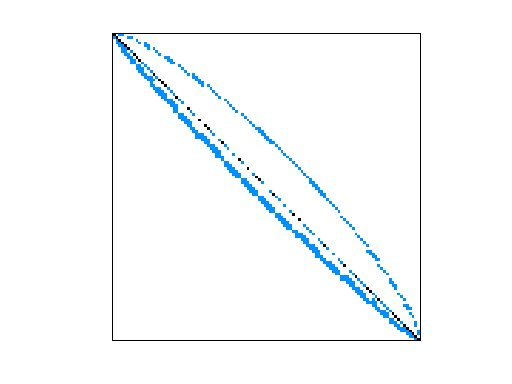
\includegraphics[width=1.1\linewidth]{figures/gre_216a/matrix.png}
		\caption{}		
	\end{subfigure}
	\quad
	\begin{subfigure}[t]{0.45\linewidth}
		\centering
		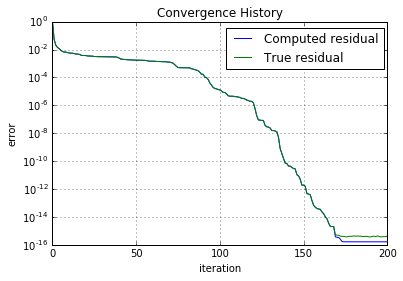
\includegraphics[width=1.15\linewidth]{figures/gre_216a/convergence_history.png}
		\caption{}
	\end{subfigure}
	\caption{Matrix HB/gre_216a and its GMRES convergence history.}\label{fig:gre_216a}
\end{figure}
\begin{figure}[h]
	\centering
	\begin{subfigure}[t]{0.45\linewidth}
		\centering
		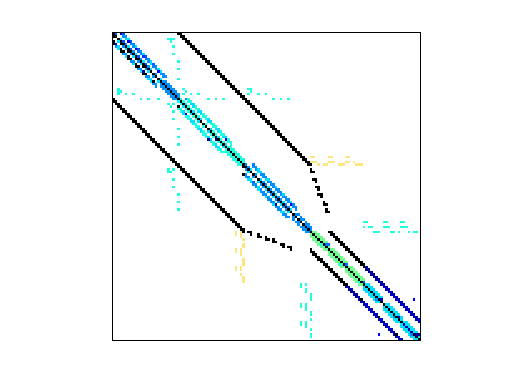
\includegraphics[width=1.1\linewidth]{figures/pores_2/matrix.png}
		\caption{}	
	\end{subfigure}
	\quad
	\begin{subfigure}[t]{0.45\linewidth}
		\centering
		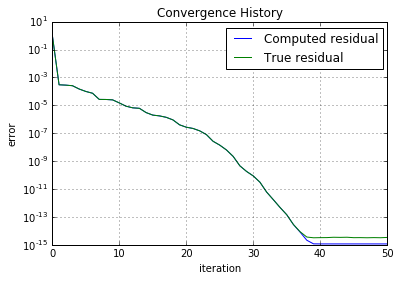
\includegraphics[width=1.15\linewidth]{figures/pores_2/convergence_history.png}
		\caption{}
	\end{subfigure}
	\caption{Matrix HB/pores_2 and its preconditioned-GMRES convergence history.}\label{fig:pores_2}	
\end{figure}





\begin{table}[ht]
\caption{Matrices used} % title of Table
\centering % used for centering table
\begin{tabular}{c c c c} % centered columns (4 columns)
\hline\hline %inserts double horizontal lines
Name & Size (n)& Non-Zeros (\%) & type \\ [0.5ex] % inserts table
%heading
\hline % inserts single horizontal line
HB/arc130 & $130$ & 0.061 & real unsymmetric \\ % inserting body of the table
Bai/lop163 & $163$ & 0.035 & real unsymmetric  \\
HB/mcca & $183$ & 0.082 & real unsymmetric  \\
Rajat/rajat14 & $180$ & 0.046 & real unsymmetric  \\
HB/fs_183_1 & $183$ & 0.030 & real unsymmetric  \\
Bai/rdb200 & $200$ & 0.028 & real unsymmetric  \\
JGD_Trefethen/Trefethen_200 & $200$ & 0.072 & real unsymmetric  \\
HB/impcol_a & $207$ & 0.013 & real unsymmetric  \\
HB/gre_216a & $216$ & 0.017 & real unsymmetric  \\
HB/steam1 & $240$ & 0.039 & real unsymmetric  \\ [1ex] % [1ex] adds vertical space
\hline %inserts single line
\end{tabular}
\label{table:nonlin} % is used to refer this table in the text
\end{table}


%\subsection{Fault, failure and error}
%The following taxonomy is used~\cite{fault_taxonomy} :
%\begin{itemize}
%\item A fault is 
%\item An error is
%\item A failure is 
%\end{itemize}
%Transient faults, \\
%Soft error, \\
%\subsection*{Notations}
%When a quantity relates to a faulty execution, a '$\sim$' is added on top of the symbol used for the same quantity in the non-faulty execution.

%\newpage


% \begin{algorithm}
% \caption{Faulty product $z \leftarrow A \cdot v$}\label{alg:faulty_product}
% \begin{algorithmic}[1]
% \For {$i = 0,..., n-1$}
% 	\State $z_i \gets 0$
% 	\For {$k = 0,..., n-1$}
%     	\If {$A_{i, k} \neq 0 \text{ and } v_k \neq 0$}
%         	\State \text{a bit flip may happen during the following operations}
%         	\State $reg_1 \xleftarrow{vulnerable} A_{i, k}$
%             \State $reg_2 \xleftarrow{vulnerable} v_k$ 
%             \State $reg_3 \xleftarrow{vulnerable} reg_1 \cdot reg_2$
%             \State $z_i \gets z_i + reg_3$
%         \EndIf
%     \EndFor
% \EndFor
% \end{algorithmic}
% \end{algorithm}

